\documentclass[11pt]{article}
\usepackage[margin=0.7in]{geometry}
\usepackage{tikz,longtable,hyperref}
\setlength{\parindent}{0pt}\setlength{\parskip}{7pt}
\begin{document}
\raggedright\sloppy
{\LARGE First-gate infrastructure failure and executable-mode correction}\\[5pt]
2026-10-30T00:15:53Z\\
Public synthetic known-answer mathematical research. Evidence observations only; no judgments, new cohort executions or qualification.

Zero executions refers to this named plan-only input, not historical experiments. Per-source software scopes are distinct and counts are never pooled.
\section*{Plan-only observations}
\begin{center}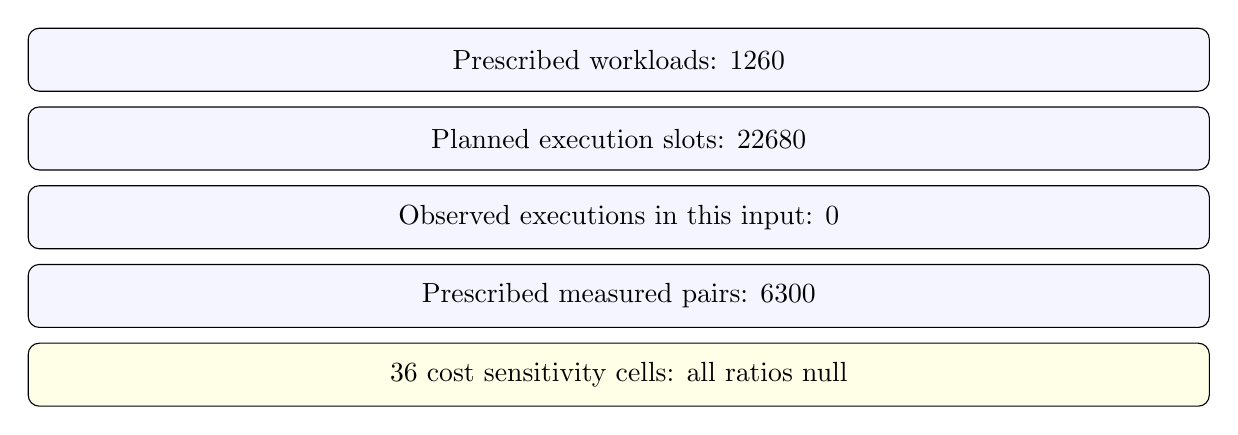
\begin{tikzpicture}
\node[draw,rounded corners,fill=blue!4,minimum width=15cm,minimum height=0.8cm] at (0,-0) {Prescribed workloads: 1260};
\node[draw,rounded corners,fill=blue!4,minimum width=15cm,minimum height=0.8cm] at (0,-1) {Planned execution slots: 22680};
\node[draw,rounded corners,fill=blue!4,minimum width=15cm,minimum height=0.8cm] at (0,-2) {Observed executions in this input: 0};
\node[draw,rounded corners,fill=blue!4,minimum width=15cm,minimum height=0.8cm] at (0,-3) {Prescribed measured pairs: 6300};
\node[draw,rounded corners,fill=yellow!10,minimum width=15cm,minimum height=0.8cm] at (0,-4) {36 cost sensitivity cells: all ratios null};
\end{tikzpicture}\end{center}
Diagram rather than a performance graph: this input contains no observed empirical ratios. Counts are read from source [plan]; no rates or uncertainty estimates are inferred.
Warmup execution slots prescribed: 3780. No empirical cost ratio is available in this snapshot. Software validation and prepared inputs do not constitute independent protocol, binary, resource or launch admission.
\section*{Scoped source observations}
\textbf{[first-attempt]} Actual first gate terminated before payload spawn. This is an infrastructure failure; no mathematical target was executed and no cost ratio was measured.\\
checkpoint\_generations: 0\\
error: "Permission denied (os error 13)"\\
mathematical\_results: 0\\
payload\_pid: null\\
phase: "failed"\\
run: "pencil-p739-20261029"\\
targets\_executed: 0\\
\textbf{[mode-correction]} A new immutable image changes only the progress executable permission. File bytes and other modes are unchanged. Offline usage checks do not invoke a workload.\\
after\_result: "Expected native Usage diagnostic before payload arguments or workload loading"\\
after\_uid1000\_exit: 1\\
before\_uid1000\_exit: 126\\
changed\_path: "/opt/isolab/recovery/isolab-criu-progress"\\
file\_bytes\_equal: true\\
new\_mode: "0755"\\
old\_mode: "0700"\\
other\_modes\_equal: true\\
solver\_executions: 0\\
\textbf{[independent-mode-review]} Independent receipt, recipe, inventory, image-readback and no-payload usage review. This verifies the identified permission correction, not a future controller run or mathematical result.\\
instrument\_bytes\_equal: true\\
recovery\_verified: false\\
registry\_digest\_active: true\\
review\_result: "pass\_metadata\_correction\_for\_identified\_eacces"\\
scientific\_qualification: false\\
stopped\_container\_never\_started: true\\
\textbf{[retry-boundary]} Retry execution and its outcome are handled separately. This report preserves the failed attempt and records no empirical ratio from a later attempt.\\
new\_empirical\_ratio: null\\
new\_solver\_observations: 0\\
report\_launched\_retries: 0\\
retry\_outcome: "pending separate observation"\\
\section*{Evidence and limits}
No software test count is an empirical target count. Missing costs stay null. Resource authorization is limited to its explicit source scope; no budget, deadline, infrastructure approval or independent review is inferred. The prior 19:06 report and its Python generator remain historical artifacts; new reports use this native renderer.
\small
\textbf{[plan]} named plan-only input; not historical experiments\\
\texttt{/\allowbreak{}home/\allowbreak{}ec2-user/\allowbreak{}crypto-pencil-signed-graph-20261029/\allowbreak{}research/\allowbreak{}pencil\_large\_prime\_20261029/\allowbreak{}validation/\allowbreak{}accounting/\allowbreak{}aggregate/\allowbreak{}actual-plan-only-summary-final.json}\\
SHA256: \texttt{9c0d055e2af7f6f79ce201b9b0c2a22691da0af55e8f6f127acec7070bb7e665}\\
\textbf{[first-attempt]} Actual first gate terminated before payload spawn. This is an infrastructure failure; no mathematical target was executed and no cost ratio was measured.\\
\texttt{/\allowbreak{}home/\allowbreak{}ec2-user/\allowbreak{}crypto-pencil-signed-graph-20261029/\allowbreak{}research/\allowbreak{}pencil\_large\_prime\_20261029/\allowbreak{}validation/\allowbreak{}runtime\_permission\_correction\_20261030/\allowbreak{}first-attempt-review.json}\\
SHA256: \texttt{6e0c4c56340da2bf3bff811eef76594819491ce563652814c7ae257f822b8998}\\
\textbf{[mode-correction]} A new immutable image changes only the progress executable permission. File bytes and other modes are unchanged. Offline usage checks do not invoke a workload.\\
\texttt{/\allowbreak{}home/\allowbreak{}ec2-user/\allowbreak{}crypto-pencil-signed-graph-20261029/\allowbreak{}research/\allowbreak{}pencil\_large\_prime\_20261029/\allowbreak{}validation/\allowbreak{}runtime\_permission\_correction\_20261030/\allowbreak{}receipt.json}\\
SHA256: \texttt{a22c525366e684e73c4559c4db6083d995109af7ccf04451baf1846a103b2a39}\\
\textbf{[independent-mode-review]} Independent receipt, recipe, inventory, image-readback and no-payload usage review. This verifies the identified permission correction, not a future controller run or mathematical result.\\
\texttt{/\allowbreak{}home/\allowbreak{}ec2-user/\allowbreak{}crypto-pencil-signed-graph-20261029/\allowbreak{}research/\allowbreak{}pencil\_large\_prime\_20261029/\allowbreak{}validation/\allowbreak{}runtime\_permission\_correction\_20261030/\allowbreak{}independent-review.json}\\
SHA256: \texttt{63a7cf1b120c18ae7c9e3b8257009a4d6aed45479133a99c5ba6af2bf824a2fa}\\
\textbf{[retry-boundary]} Retry execution and its outcome are handled separately. This report preserves the failed attempt and records no empirical ratio from a later attempt.\\
\texttt{/\allowbreak{}home/\allowbreak{}ec2-user/\allowbreak{}crypto-pencil-signed-graph-20261029/\allowbreak{}research/\allowbreak{}pencil\_large\_prime\_20261029/\allowbreak{}validation/\allowbreak{}runtime\_permission\_correction\_20261030/\allowbreak{}report-scope.json}\\
SHA256: \texttt{271455d43d7e6b97338dd21b3b79bfb00bf69fd008fec8ee437040aade6590cd}\\
\end{document}
